% TEMPLATE PARA TCC 
% Unidade Acadêmcia de Belo Jardim (UABJ) - UFRPE
% Belo Jardim - 2025
% Moisés Tavares

% Baseado no projeto: 
% http://tcc.tsi.gp.utfpr.edu.br/paginas/modelos-latex-da-utfpr
% De: Diego Marczal e Michael Vornes
% Template para TCC - Universidade Federal do Pará
% De: Sérgio Custódio e Kelvin Pinheiro

\documentclass[a4paper, oneside, english, brazil, 12pt]{tccufrpe}
% oneside = Impresssão apenas na frente
% twoside = Impressão em frente e verso
\usepackage{setspace}

%-----------------------------------------------------------------------
% PREENCHER OS CAMPOS ABAIXO:
%-----------------------------------------------------------------------

\titulo{Avaliação do Impacto do ChatGPT na Aprendizagem de Heap e Tabelas Hash em Algoritmos e Estruturas de Dados}
%\subtitulo{subtítulo (se houver)} % Se não houver, deixar comentado (%)

\autor{Elias Vitor da Silva} 

\local{Belo Jardim} % separar por vírgula, caixa baixa
\data{09}{2025}
\diadefesa{02}

\projeto{Trabalho de Conclusão de Curso}
% Preencher com uma das opções: Projeto / Relatório dos resultados parciais / Trabalho de conclusão de curso

\tituloTCC{Avaliação do Impacto do ChatGPT na Aprendizagem de Heap e Tabelas Hash em Algoritmos e Estruturas de Dados}

% Dados do Orientador
\orientador{Prof. Dr. Waldemar Neto} % Para orientadora, usar opção abaixo
%\orientador[Orientadora:]{Profa. Nome completo da orientadora}
\instOrientador{Universidade Federal Rural de Pernambuco}

% Dados do Coorientador
% Se não houver, será necessário comentar o trecho no arquivo "tccufrpe.cls" (linhas 329-331), além do trecho abaixo
\coorientador{(Se houver) Nome completo do (a) coorientador (a)} % Para coorientadora, usar opção abaixo
%\coorientador[Coorientadora:]{Profa. Nome completo da coorientadora}


% Dados da banca
\nomePrimeiromembro{Prof. D.Sc. Texto Texto Texto (Examinador Interno)}
\instPrimeiromembro{Universidade Federal Rural de Pernambuco}
 
\nomeSegundomembro{Prof. D.Sc. Texto Texto Texto (Examinador Externo)}
\instSegundomembro{Universidade Texto Texto}

% Para incluir um terceiro membro na banca, será necessário "descomentar" o trecho no arquivo "tccufrpe.cls" (linhas 341-343)
%\nomeTerceiromembro{Prof. Nome do terceiro Avaliador (se houver)}
%\tituloTerceiromembro{Titulação}
%\instTerceiromembro{Instituição (SIGLA)}

%-----------------------------------------------------------------------
% ESTRUTURA DO DOCUMENTO (cuidado ao realizar modificações)
%-----------------------------------------------------------------------

\begin{document}
	\pretextual
	\imprimircapa
    \imprimirfolhaderosto{}
    %\includepdf{fichacatalográfica.pdf}
    
    \imprimirfolhadeaprovacao{}
    % Este comando insere uma Folha de aprovação em branco, elemento obrigatório da NBR 14724/2011. Você pode utilizar este modelo até a aprovação do trabalho. Após isso, substitua todo o conteúdo deste arquivo por uma imagem da página assinada pela banca com o comando abaixo:
    %\includepdf{folhadeaprovacao_final.pdf}

    % DEDICATÓRIA

\begin{dedicatoria}

Dedico este trabalho à minha família, pelo apoio constante, pela confiança e pelo incentivo durante toda a minha trajetória acadêmica.

\end{dedicatoria}
 % opcional
	% AGRADECIMENTOS

\begin{agradecimentos}[AGRADECIMENTOS]

Agradeço, primeiramente, à minha família, pelo apoio, incentivo e compreensão ao longo de toda a minha trajetória acadêmica. Sua presença foi essencial para que eu pudesse superar os desafios encontrados durante a graduação e manter o compromisso com a conclusão deste trabalho.

Agradeço também ao meu orientador, aos professores e colegas que contribuíram direta ou indiretamente para minha formação, compartilhando conhecimentos, experiências e orientações importantes para o desenvolvimento desta pesquisa. Estendo meus agradecimentos à Universidade Federal Rural de Pernambuco, especialmente à Unidade Acadêmica de Belo Jardim, pela oportunidade de formação e pelo ambiente acadêmico que possibilitou a realização deste Trabalho de Conclusão de Curso.

\end{agradecimentos}
	% EPÍGRAFE

\begin{epigrafe}

\OnehalfSpacing
Aprender não consiste apenas em obter respostas, mas em desenvolver o pensamento crítico, compreender problemas, avaliar caminhos e construir soluções.

\end{epigrafe}
 % opcional

    \OnehalfSpacing
    % RESUMO

\begin{resumo}[RESUMO (OBRIGATÓRIO)]
\begin{Spacing}{1.5}

Uma competência fundamental na formação em Computação é a capacidade de compreender, implementar e selecionar estruturas de dados adequadas para diferentes problemas. Nesse contexto, o avanço de ferramentas de inteligência artificial generativa, como o ChatGPT, tem provocado discussões sobre seus possíveis efeitos na aprendizagem de estudantes em disciplinas de programação. Este trabalho investiga o impacto do uso do ChatGPT na aprendizagem de alunos da disciplina de Algoritmos e Estruturas de Dados, com foco nos conteúdos de Heap e Tabelas Hash. A pesquisa toma como base metodológica um estudo experimental aplicado a estruturas de dados em contexto de graduação, adaptando seu recorte para os tópicos selecionados neste trabalho. A proposta envolve a realização de atividades práticas com grupos de estudantes submetidos a diferentes condições de uso do ChatGPT, permitindo comparar evidências de aprendizagem por meio de questionários, desempenho acadêmico e análise de similaridade de código. Com isso, busca-se observar se o uso da ferramenta influencia a compreensão conceitual e prática dos conteúdos, bem como se contribui para maior semelhança entre as soluções produzidas. Espera-se que os resultados contribuam para a discussão sobre o uso pedagógico de inteligência artificial generativa em cursos de Computação e para o planejamento de atividades avaliativas mais adequadas ao cenário atual.
\end{Spacing}
\vspace{1cm}
\textbf{Palavras-chave}: ChatGPT, inteligência artificial generativa, algoritmos e estruturas de dados, Heap, tabelas hash, aprendizagem.

\end{resumo}

% OBSERVAÇÕES:

% Escolha de 3 a 5 palavras ou termos que descrevam bem o seu trabalho .
% As palavras-chave são separadas por vírgula.


	% ABSTRACT

\begin{resumo}[ABSTRACT (OBRIGATÓRIO)]
\begin{Spacing}{1.5}

An essential competency in Computing education is the ability to understand, implement, and select suitable data structures for different problems. In this context, the advance of generative artificial intelligence tools, such as ChatGPT, has raised discussions about their possible effects on students' learning in programming courses. This work investigates the impact of ChatGPT usage on students' learning in the Data Structures and Algorithms course, focusing on Heap and Hash Table topics. The research is methodologically inspired by an experimental study conducted with undergraduate students in data structures, adapting its scope to the topics selected in this work. The proposed study involves practical activities with groups of students under different ChatGPT usage conditions, allowing the comparison of learning evidence through questionnaires, academic performance, and code similarity analysis. Thus, this work seeks to observe whether the use of the tool influences students' conceptual and practical understanding of the topics, as well as whether it contributes to greater similarity among the produced solutions. The expected contribution is to support discussions about the pedagogical use of generative artificial intelligence in Computing courses and the design of assessment activities more suitable for the current educational scenario.

\end{Spacing}

\vspace{1cm}
\textbf{Keywords}: ChatGPT, generative artificial intelligence, data structures and algorithms, Heap, hash tables, learning.

\end{resumo}

% OBSERVAÇÕES:

% Escolha de 3 a 5 palavras ou termos que descrevam bem o seu trabalho .
% As palavras-chave são separadas por vírgula.


	
    \listoffigures*
    \newpage
    \listoftables*
    %\listofalgorithms
    % LISTA DE ABREVIATURAS E SIGLAS

\begin{center}
    \textbf{LISTA DE ABREVIATURAS E SIGLAS (OPCIONAL)}
    \vspace{1cm}
\end{center}

\begin{table}[h]
    \begin{tabular}{lcl}
        ABNT & \hspace{0.5cm} & Associação Brasileira de Normas Técnicas \\
        DSA & \hspace{0.5cm} & Data Structures and Algorithms \\
        IA & \hspace{0.5cm} & Inteligência Artificial \\
        TCC & \hspace{0.5cm} & Trabalho de Conclusão de Curso \\
        UABJ & \hspace{0.5cm} & Unidade Acadêmica de Belo Jardim \\
        UFRPE & \hspace{0.5cm} & Universidade Federal Rural de Pernambuco
    \end{tabular}
\end{table}

% OBSERVAÇÃO:
% Incluir em ordem alfabética
    % LISTA DE SÍMBOLOS

\begin{center}
    \textbf{LISTA DE SÍMBOLOS}
    \vspace{1cm}
\end{center}

\begin{table}[h]
    \begin{tabular}{lcl}
        $H_0$ & \hspace{0.5cm} & Hipótese nula \\
        $H_1$ & \hspace{0.5cm} & Hipótese alternativa \\
        $n$ & \hspace{0.5cm} & Tamanho da amostra \\
        $O(\cdot)$ & \hspace{0.5cm} & Notação assintótica de complexidade \\
        $p$ & \hspace{0.5cm} & Valor de significância estatística \\
        $\delta$ & \hspace{0.5cm} & Tamanho de efeito de Cliff
    \end{tabular}
\end{table}
    \tableofcontents*
    \newpage
    
	\textual
	% INTRODUÇÃO

\chapter{INTRODUÇÃO}
\label{chap:introducao}

Algoritmos e Estruturas de Dados constituem uma área fundamental na formação em Computação, pois fornecem a base para organizar, processar e recuperar informações de maneira eficiente \cite{leblanc2015se2014,cormen2022introduction}. Entre os conteúdos dessa disciplina, Heap e Tabelas Hash são estruturas amplamente utilizadas e exigem articulação entre teoria, análise de complexidade e implementação prática \cite{cormen2022introduction}.

Nos últimos anos, ferramentas de inteligência artificial generativa, como o ChatGPT, passaram a integrar o cotidiano dos estudantes de programação, auxiliando na explicação de conceitos, na geração de exemplos e na sugestão de soluções \cite{baidoo2023education,rahman2023education,garcia2025programming}. Ao mesmo tempo, seu uso suscita questionamentos sobre autonomia, pensamento crítico e possível dependência de respostas prontas \cite{dwivedi2023chatgpt,delikoura2025superficial,qin2023general}, especialmente em disciplinas que exigem raciocínio lógico e a implementação de algoritmos.

Diante desse cenário, o problema investigado neste trabalho foi formulado por meio da seguinte questão de pesquisa: \textit{o uso do ChatGPT durante atividades práticas de Algoritmos e Estruturas de Dados altera o desempenho dos estudantes, medido pela pontuação nos questionários sobre Heap e Tabelas Hash, quando comparadas as condições com e sem a ferramenta?} Essa questão insere-se em investigações recentes sobre o impacto do ChatGPT em programação e em disciplinas de estruturas de dados \cite{jamie2024dsa,kosar2024chatgpt}.

Este Trabalho de Conclusão de Curso foi motivado por um artigo recentemente aprovado no Congresso Brasileiro de Engenharia de Software (CBSoft) \cite{neto2026chatgpt}, que investiga o impacto do ChatGPT na aprendizagem de Algoritmos e Estruturas de Dados. A presente pesquisa dá continuidade a essa linha de investigação, com foco nos conteúdos de Heap e Tabelas Hash.

\section{Objetivos}

\subsection{Objetivo geral}

O objetivo geral deste trabalho é analisar se o uso do ChatGPT durante atividades práticas influencia o desempenho dos estudantes, medido pela pontuação nos questionários sobre Heap e Tabelas Hash.

\subsection{Pergunta de pesquisa}

A partir do objetivo geral, formula-se a seguinte pergunta de pesquisa, alinhada ao problema apresentado na seção anterior: \textit{o uso do ChatGPT durante atividades práticas de Algoritmos e Estruturas de Dados altera o desempenho dos estudantes, medido pela pontuação nos questionários sobre Heap e Tabelas Hash, quando comparadas as condições com e sem a ferramenta?}

\subsection{Objetivos específicos}

Os objetivos específicos são:

\begin{itemize}
    \item caracterizar a participação e o perfil dos estudantes quanto ao uso prévio de IA generativa;
    \item comparar o desempenho nos questionários entre as condições com e sem uso do ChatGPT;
    \item discutir os resultados à luz da literatura e das limitações do desenho experimental adotado.
\end{itemize}

Para atingir esses objetivos, adota-se um desenho experimental com grupos cruzados, no qual cada grupo utiliza a ferramenta em um tópico e não a utiliza no outro. O desempenho é operacionalizado como a pontuação obtida em questionários objetivos aplicados ao final de cada atividade prática, sem apoio do ChatGPT.


	% FUNDAMENTAÇÃO TEÓRICA--------------------------------------------------------

\chapter{REFERENCIAL TEÓRICO}
\label{chap:referencial-teorico}

Demonstrar os assuntos relevantes à temática da pesquisa proposta, com base em publicações técnicas e científicas, sobretudo artigos científicos nacionais e internacionais, preferencialmente aqueles publicados nos últimos 10 anos. Deve contemplar, de maneira clara e objetiva, os elementos conceituais e a fundamentação teórica e científica que sejam importantes para respaldar a pesquisa, bem como servir de apoio para os procedimentos metodológicos inerentes ao tema proposto e para a interpretação dos resultados. 

As citações diretas longas (com mais de três linhas) devem constituir um parágrafo independente, recuado 4 cm da margem esquerda, justificado, fonte Arial ou Times New Roman, tamanho 10 e espaçamento 1 (simples) entre linhas, dispensando as aspas. É preciso indicar, obrigatoriamente, a fonte consultada, com o(s) nome(s) do(s) autor(es), ano de publicação e página. Caso o original contenha uma citação com uso de aspas, empregar aspas simples.

\begin{adjustwidth}{4cm}{}
    \SingleSpacing
    \small
    A NBR 10520 (ABNT, 2002b) recomenda, para as citações longas, o uso de recuo sem aspas; no entanto, quando houver necessidade de, no meio de uma citação longa, fazer-se uma interrupção para introduzir um comentário do autor, é preferível fechar a citação com aspas, fazer o comentário e abrir uma nova citação com aspas. (FRANÇA; VASCONCELLOS, 2013, p. 137).
    \vspace{0.4cm}
\end{adjustwidth}

\noindent \textcolor{cyan}{(No corpo do trabalho, tanto nas ilustrações como nas tabelas, a identificação aparece na parte superior. Na parte inferior, indica-se a fonte consultada – obrigatório, mesmo que seja produção de própria autoria conforme exemplo acima.)
\\
(A numeração das ilustrações deve ser sequencial (Figura \ref{fig:FIGURA1}, Figura \ref{fig:FIGURA2}), de acordo com a ordem que aparece no texto. Ao longo do texto, os títulos das ilustrações devem ser escritos da mesma forma e com os mesmos destaques gráficos (negrito, itálico, sublinhado, etc) que na lista de ilustrações. O mesmo acontece para as tabelas.)
}

\begin{figure}[!ht]
    \SingleSpacing
	\centering
	\caption{Nuvem de Tags dos PPCs das licenciaturas em Ciências Biológicas, Física e Química da UFRPE}
	\includegraphics[scale=1.5]{Figuras/Figura1.png}
    	\caption*{Fonte: Silva, 2019.}
	\label{fig:FIGURA1}
\end{figure}

Este capítulo também pode conter subdivisões conforme as peculiaridades de cada pesquisa, bem como a necessidade do autor. Neste caso, os subtítulos, também chamados de seções secundárias, devem ter numeração progressiva e seguindo o título principal; separado por um espaço 1,5 do texto que o precede e do que o sucede. Todos os itens precisam ser indicados no sumário.

\section{Título}
\label{sec:Título}

Texto texto texto texto texto texto texto texto texto texto texto texto texto texto texto texto texto texto texto texto texto texto texto texto texto texto texto texto texto.

Texto texto texto texto texto texto texto texto texto texto texto texto texto texto texto texto texto texto texto texto texto texto texto texto texto texto texto texto texto.

\subsection{Título}
\label{subsec:Título}

Texto texto texto texto texto texto texto texto texto texto texto texto texto texto texto texto texto texto texto texto texto texto texto texto texto texto texto texto texto texto texto.

\subsubsection{Título}
\label{subsubsec:Título}

Texto texto texto texto texto texto texto texto texto texto texto texto texto texto.

\begin{figure}[!ht]
    \SingleSpacing
	\centering
	\caption{Título título título}
	\includegraphics[scale=0.3]{Figuras/Figura2.PNG}
    	\caption*{Fonte: O autor, ano.}
	\label{fig:FIGURA2}
\end{figure}

Texto texto texto texto texto texto texto texto texto texto texto texto texto texto texto texto texto.

\subsubsubsection{Título}
\label{subsubsubsec:Título}


Texto texto texto texto texto texto texto texto texto texto texto texto texto texto texto texto texto.
	% METODOLOGIA

\chapter{METODOLOGIA}
\label{chap:metodologia}

Este capítulo descreve os procedimentos metodológicos adotados para investigar o impacto do uso do ChatGPT no desempenho dos estudantes em Algoritmos e Estruturas de Dados, com foco em Heap e Tabelas Hash. O estudo adota um desenho experimental com grupos cruzados, no qual as condições de uso da ferramenta são invertidas entre os dois tópicos investigados.

\section{Caracterização da Pesquisa}
\label{sec:caracterizacao-pesquisa}

A pesquisa caracteriza-se como um estudo empírico em contexto educacional, com abordagem quantitativa e desenho comparativo. O objetivo é observar se o uso do ChatGPT em atividades práticas de programação influencia o desempenho dos estudantes nos conteúdos trabalhados. Para isso, adota-se um desenho experimental com dois grupos e condições invertidas de uso da ferramenta entre os tópicos Heap e Tabelas Hash \cite{wohlin2012experimentation}.

Neste estudo, o \textbf{desempenho} é operacionalizado como a pontuação obtida por cada estudante em questionários objetivos de múltipla escolha, aplicados ao final de cada atividade prática, sem apoio do ChatGPT. O questionário de Heap continha 20 questões e o de Tabelas Hash, 21. A pontuação corresponde ao número de acertos, com o mesmo peso por questão, resultando em escalas de 0 a 20 e de 0 a 21, respectivamente. Essa medida permite comparar o desempenho nas condições com e sem uso da ferramenta durante as implementações.

\section{Contexto e Participantes}
\label{sec:contexto-participantes}

O estudo foi conduzido na disciplina de Algoritmos e Estruturas de Dados, vinculada ao curso de Engenharia da Computação da Universidade Federal Rural de Pernambuco, na Unidade Acadêmica de Belo Jardim, no primeiro semestre letivo de 2026 (2026.1). A disciplina integra tipicamente o terceiro período da grade curricular e tem, como formação prévia esperada, conteúdos de Programação Orientada a Objetos (ou equivalente). O experimento ocorreu no final da disciplina. As atividades práticas foram implementadas em Java, linguagem adotada no componente curricular.

Os participantes foram estudantes regularmente matriculados no período de aplicação do estudo. A participação foi voluntária, precedida da apresentação dos objetivos da pesquisa e do aceite por meio do termo de consentimento livre e esclarecido (TCLE). Como incentivo acadêmico, a participação nas atividades experimentais valeu 1 ponto na disciplina. Os dados analisados foram tratados de forma agregada ou anonimizada, preservando a confidencialidade dos participantes. Ao todo, 28 estudantes responderam ao formulário inicial vinculado ao TCLE; desses, 25 integraram a distribuição experimental nos grupos --- três estudantes que responderam ao formulário não compareceram no dia da alocação aos grupos e, portanto, não participaram das atividades experimentais.

\section{Conteúdos Investigados}
\label{sec:conteudos-investigados}

Este TCC concentra-se nos conteúdos de Heap e Tabelas Hash, escolhidos por combinarem fundamentos conceituais, análise de complexidade e desafios de implementação relevantes na formação em Computação \cite{cormen2022introduction}. Heap foi o primeiro conteúdo trabalhado no experimento; Tabelas Hash, o segundo, com inversão das condições de uso do ChatGPT entre os grupos.

\section{Hipótese da Pesquisa}
\label{sec:hipotese-pesquisa}

A investigação considera uma única hipótese nula, associada ao desempenho nos questionários após as atividades práticas:

\begin{itemize}
    \item $H_{0}$: não há diferença significativa no desempenho dos estudantes --- medido pela pontuação nos questionários --- quando comparamos condições com e sem uso do ChatGPT nas atividades práticas de Algoritmos e Estruturas de Dados.
\end{itemize}

A hipótese $H_{0}$ é avaliada por meio das pontuações obtidas nos questionários aplicados após cada atividade prática, comparando o desempenho dos estudantes em Heap e Tabelas Hash sob cada condição experimental. A análise estatística considera o tamanho da amostra e a distribuição dos dados, empregando testes não paramétricos quando necessário \cite{kitchenham2019statistical,sheskin2003handbook}.

\section{Desenho Experimental}
\label{sec:desenho-experimental}

O desenho experimental é organizado em três momentos principais: etapa inicial, atividade de Heap e atividade de Tabelas Hash. Em cada atividade prática, a avaliação do desempenho foi realizada por meio de um questionário aplicado ao final da implementação, sem uso do ChatGPT. A Figura \ref{fig:fluxo-metodologia} apresenta uma visão geral do processo. Nela, a etapa experimental inicia com 25 estudantes distribuídos nos grupos; a análise comparativa final considera apenas os 20 participantes com participação completa, isto é, que cumpriram todas as etapas da pesquisa --- do formulário de perfil até o último questionário.

\begin{figure}[!ht]
    \SingleSpacing
    \centering
    \caption{Visão geral do processo experimental.}
    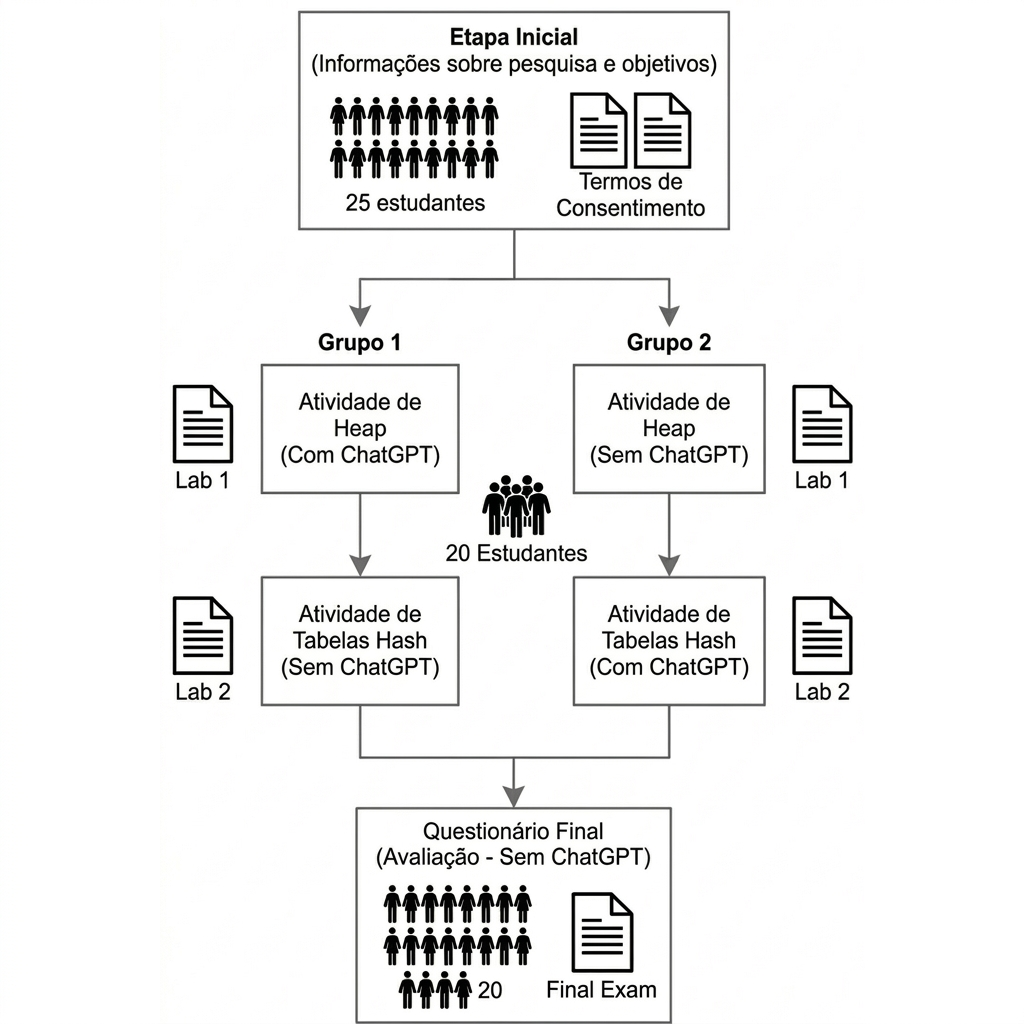
\includegraphics[width=\textwidth]{Figuras/fluxo-metodologia.png}
    \vspace{-0.4cm}
    \caption*{Fonte: Elaboração própria.}
    \label{fig:fluxo-metodologia}
\end{figure}

Na etapa inicial, os estudantes foram informados sobre a pesquisa, seus objetivos, as atividades previstas e as condições de participação. Antes do início das atividades experimentais, os participantes assinaram o termo de consentimento livre e esclarecido (TCLE) e responderam a perguntas sobre familiaridade prévia e frequência de uso de ferramentas de inteligência artificial generativa, especialmente em atividades de programação. Ao todo, 28 estudantes responderam a esse formulário, autorizando o uso dos dados exclusivamente para fins acadêmicos. A Tabela \ref{tab:perfil-ia} resume o perfil desses 28 respondentes quanto ao conhecimento e ao uso dessas ferramentas.

\begin{table}[!ht]
    \centering
    \caption{Perfil dos participantes quanto ao uso de IA generativa ($n = 28$, formulário inicial)}
    \label{tab:perfil-ia}
    \begin{tabular}{l c c}
        \hline
        \textbf{Indicador} & \textbf{$n$} & \textbf{Percentual} \\
        \hline
        Já conhecia IA generativa & 28 & 100,0\% \\
        \hline
        \multicolumn{3}{l}{\textit{Frequência de uso geral}} \\
        Mais de uma vez ao dia & 10 & 35,7\% \\
        Uma vez ao dia & 2 & 7,1\% \\
        Várias vezes na semana & 9 & 32,1\% \\
        Algumas vezes na semana & 7 & 25,0\% \\
        \hline
        \multicolumn{3}{l}{\textit{Uso em atividades de programação}} \\
        Sempre & 1 & 3,6\% \\
        Quase sempre & 25 & 89,3\% \\
        Raramente & 2 & 7,1\% \\
        \hline
    \end{tabular}

    \vspace{0.2cm}
    \caption*{Fonte: Elaboração própria, com base no termo de consentimento.}
\end{table}

Conforme a Tabela \ref{tab:perfil-ia}, todos os respondentes já possuíam conhecimento prévio sobre ferramentas de IA generativa e a maioria declarou utilizá-las com frequência em atividades de programação. Em seguida, os 25 participantes que integraram o experimento foram distribuídos aleatoriamente em dois grupos de tamanho semelhante --- Grupo 1 com 12 estudantes e Grupo 2 com 13 --- com condições invertidas de uso do ChatGPT:

\begin{itemize}
    \item \textbf{Grupo 1:} utilizou o ChatGPT na atividade prática de Heap e não utilizou a ferramenta na atividade prática de Tabelas Hash.
    \item \textbf{Grupo 2:} não utilizou o ChatGPT na atividade prática de Heap e utilizou a ferramenta na atividade prática de Tabelas Hash.
\end{itemize}

Esse arranjo, conhecido como desenho com grupos cruzados, permite que cada tópico seja estudado sob as duas condições experimentais, reduzindo o efeito de diferenças sistemáticas entre os conteúdos. Cada participante vivenciou uma atividade com a ferramenta e outra sem ela. A Tabela \ref{tab:resumo-participacao} resume a participação e as perdas amostrais ao longo do experimento.

\begin{table}[!ht]
    \centering
    \caption{Resumo da participação no experimento}
    \label{tab:resumo-participacao}
    \begin{tabular}{l c}
        \hline
        \textbf{Indicador} & \textbf{Quantidade} \\
        \hline
        Estudantes distribuídos nos grupos & 25 \\
        Participação completa (Heap e Tabelas Hash) & 20 \\
        Desistentes & 5 \\
        Grupo 1 com participação completa & 9 \\
        Grupo 2 com participação completa & 11 \\
        \hline
    \end{tabular}

    \vspace{0.2cm}
    \caption*{Fonte: Elaboração própria, com base na planilha de coleta do experimento.}
\end{table}

Dos 25 estudantes distribuídos, cinco não concluíram todas as etapas e foram excluídos da análise comparativa (três no Grupo 1 e duas no Grupo 2), resultando em 20 participantes com participação completa.

O experimento foi realizado em dois encontros distintos, cada um com duração aproximada de duas horas, abrangendo aula teórica, atividade prática e aplicação do questionário. No primeiro encontro, os participantes assistiram à aula teórica de Heap e, na sequência, realizaram a implementação prática em ambiente de laboratório e responderam ao questionário objetivo correspondente. As condições de uso do ChatGPT seguiram a divisão dos grupos descrita anteriormente. No grupo autorizado a usar a ferramenta, foi permitido o acesso à interface web do ChatGPT na versão gratuita, com seleção automática de modelo e uso livre, sem roteiro prévio de \textit{prompts}; no grupo sem ChatGPT, os estudantes puderam consultar materiais didáticos, anotações e documentação, mas não ferramentas de IA generativa. O docente e monitores acompanharam o laboratório para reforçar o cumprimento das condições. Ao término da atividade, todos responderam ao questionário sobre Heap, sem apoio do ChatGPT.

Aproximadamente 15 dias depois, ocorreu o segundo encontro, dedicado a Tabelas Hash, com a mesma estrutura (aula teórica, implementação prática e questionário), porém com as condições de uso do ChatGPT invertidas entre os grupos.

\section{Instrumentos e Materiais}
\label{sec:instrumentos-materiais}

As atividades práticas foram disponibilizadas por meio de repositórios que contêm código-base e métodos a serem implementados. Essa estrutura padronizou as tarefas e garantiu que todos os estudantes trabalhassem sobre os mesmos requisitos. O código-base continha apenas a estrutura necessária para orientar a implementação, sem fornecer diretamente a solução dos métodos avaliados.

O instrumento de avaliação foi composto por questionários objetivos de múltipla escolha (itens fechados). As questões foram selecionadas aleatoriamente a partir de bancos públicos de questões de entrevista técnica da plataforma Sanfoundry, alinhadas aos conteúdos de Heap e Tabelas Hash\footnote{Heapsort: \texttt{https://www.sanfoundry.com/heapsort-multiple-choice-questions-answers-mcqs/}. Hash tables (chaining): \texttt{https://www.sanfoundry.com/hash-tables-chaining-binary-trees-multiple-choice-questions-answers-mcqs/}.}. Cada acerto vale um ponto; a pontuação final de cada questionário é a soma dos acertos (0 a 20 em Heap; 0 a 21 em Tabelas Hash). Em ambos os casos, o uso do ChatGPT não foi permitido durante a aplicação do instrumento. Os questionários medem desempenho por reconhecimento e resposta a itens objetivos, e não pretendem capturar, por si sós, toda a profundidade da aprendizagem prática.

Os materiais do experimento, os enunciados das atividades, os instrumentos e os scripts de análise estatística estão disponíveis em repositório público no GitHub\footnote{\url{https://github.com/hellyaxs/MW-CL-pesquisa-tcc}}.

\section{Procedimentos de Coleta de Dados}
\label{sec:procedimentos-coleta}

A coleta de dados seguiu a sequência definida no desenho experimental. Inicialmente, os participantes receberam orientações sobre a pesquisa e foram distribuídos nos dois grupos. Em seguida, para o conteúdo de Heap, assistiram à aula teórica, realizaram a atividade prática sob a condição de uso do ChatGPT definida para seu grupo e responderam ao questionário correspondente, sem apoio da ferramenta.

Depois da conclusão dessa etapa, os estudantes participaram da aula teórica de Tabelas Hash, realizaram a atividade prática sob a condição invertida de uso do ChatGPT e responderam ao questionário sobre esse conteúdo, também sem apoio da ferramenta.

Os dados utilizados na análise comparativa foram as pontuações dos questionários de Heap e Tabelas Hash dos participantes com participação completa --- aqueles que cumpriram todas as etapas da pesquisa, desde o formulário de perfil até o último questionário. Foram excluídos da análise comparativa os cinco estudantes que não concluíram todas as etapas, embora parte deles tenha participado da etapa de Heap.

\section{Procedimentos de Análise dos Dados}
\label{sec:procedimentos-analise}

A análise dos dados foi organizada para avaliar a hipótese $H_{0}$. As pontuações de Heap e de Tabelas Hash foram reorganizadas por condição experimental --- com ChatGPT e sem ChatGPT --- e não por grupo de alocação inicial, conforme o desenho com grupos cruzados. A comparação inferencial principal considerou todas as pontuações de cada condição, totalizando 20 observações por condição na amostra completa. As pontuações foram analisadas na escala original de número de acertos, sem conversão para percentual ou outra normalização entre os questionários; essa diferença de escala (máximos 20 e 21) deve ser considerada na interpretação da comparação agregada.

Foram calculadas estatísticas descritivas das pontuações, incluindo média, mediana, desvio padrão, valores mínimo e máximo, tanto na comparação agregada entre condições quanto, de forma exploratória, separadas por conteúdo. Em seguida, verificou-se a distribuição dos dados por meio do teste de Shapiro--Wilk, como forma de avaliar a normalidade das pontuações em cada condição experimental.

Embora os resultados do teste de Shapiro--Wilk tenham indicado desvio significativo da normalidade em uma das condições, optou-se pela utilização do teste não paramétrico de Mann--Whitney U para a comparação agregada entre as pontuações com e sem uso do ChatGPT. Essa escolha foi motivada pelo tamanho reduzido da amostra, uma vez que testes não paramétricos tendem a apresentar maior robustez em estudos com número limitado de participantes \cite{kitchenham2019statistical,sheskin2003handbook}. A análise principal trata as pontuações reorganizadas por condição como duas amostras a serem comparadas quanto ao desempenho sob cada regime de uso da ferramenta. Reconhece-se, contudo, que o desenho com grupos cruzados produz, no nível do participante, um par de observações (uma com ChatGPT e outra sem); a opção pelo Mann--Whitney U agregado privilegiou a comparação entre condições na forma em que a hipótese $H_{0}$ foi formulada, em detrimento de um teste estritamente pareado, o que constitui uma limitação metodológica a ser considerada na interpretação dos resultados.

Os procedimentos descritivos e inferenciais foram executados em Python, com apoio da biblioteca SciPy para os testes de Shapiro--Wilk e de Mann--Whitney U, além do cálculo do Cliff's Delta implementado a partir das pontuações reorganizadas por condição.

Além da verificação da significância estatística, também foi calculado o coeficiente Cliff's Delta sobre a comparação agregada entre condições, com o objetivo de estimar a magnitude da diferença observada. Enquanto o teste de Mann--Whitney U permite verificar a existência de diferenças estatisticamente significativas, o Cliff's Delta complementa essa análise ao quantificar a intensidade do efeito encontrado. Para interpretação, adotaram-se os limiares propostos por Romano et al., conforme reportado por Kitchenham et al.: $| \delta | < 0{,}147$ indica efeito negligível; entre $0{,}147$ e $0{,}33$, pequeno; entre $0{,}33$ e $0{,}474$, médio; e acima de $0{,}474$, grande \cite{kitchenham2019statistical}.

	% RESULTADOS

\chapter{RESULTADOS E DISCUSSÕES}
\label{chap:resultados}

Neste capítulo do trabalho, são apresentados os resultados obtidos com as análises, conforme a metodologia aplicada, os dados disponíveis e com base na fundamentação teórica. Importante expor, ainda, as discussões de tais resultados, destacando qual foi a sua contribuição sobre a temática abordada.


	% CONCLUSÕES

\chapter{CONCLUSÕES}
\label{chap:conclusoes}

Este Trabalho de Conclusão de Curso investigou o impacto do uso do ChatGPT na compreensão de estudantes da disciplina de Algoritmos e Estruturas de Dados, com foco nos conteúdos de Heap e Tabelas Hash. O estudo foi conduzido em contexto de graduação em Engenharia da Computação, adotando um desenho experimental com grupos cruzados e questionários objetivos aplicados ao final de cada atividade prática.

Em relação ao objetivo geral proposto, os resultados indicam que o uso do ChatGPT durante as atividades práticas não produziu diferença estatisticamente significativa na compreensão dos conteúdos, medida pelos questionários de Heap e Tabelas Hash. Na comparação agregada entre as condições com e sem uso da ferramenta, a diferença entre as médias foi de apenas 0,15 ponto, o teste de Mann-Whitney U não permitiu rejeitar a hipótese $H_{0}$ ($p = 1{,}000$) e o Cliff's Delta indicou efeito negligível ($\delta = -0{,}003$). Análises separadas por tópico e o teste de Wilcoxon pareado ($p = 0{,}717$) também não identificaram diferenças significativas. Assim, no contexto analisado, não há evidências empíricas de que o ChatGPT tenha alterado de forma mensurável a compreensão avaliada pelo instrumento utilizado.

Esses achados convergem com estudos que também não identificaram impacto significativo do ChatGPT no desempenho de estudantes em disciplinas de programação e estruturas de dados \cite{kosar2024chatgpt}. Ao mesmo tempo, a interpretação dos resultados deve considerar limitações importantes. A amostra final compreendeu 20 participantes, após cinco desistências; o questionário avaliou principalmente compreensão conceitual por meio de questões objetivas; e a alta familiaridade prévia dos estudantes com IA generativa, especialmente em programação, pode ter atenuado diferenças entre as condições experimentais.

Do ponto de vista educacional, a ausência de diferença significativa não deve ser interpretada como prova de neutralidade do ChatGPT para a aprendizagem. A ferramenta pode influenciar autonomia, dependência e engajamento cognitivo de formas não capturadas pelo instrumento adotado \cite{kosmyna2025brain,delikoura2025superficial}. Ainda assim, os resultados reforçam a necessidade de cautela ao assumir que o uso do ChatGPT em atividades práticas, por si só, altera a compreensão dos conteúdos de Heap e Tabelas Hash no curto prazo.

Como desdobramentos futuros, sugere-se ampliar o tamanho amostral, empregar instrumentos que contemplem diferentes dimensões da aprendizagem, investigar efeitos de longo prazo e comparar estratégias de mediação docente no uso da ferramenta. Também seria relevante replicar o estudo em outros tópicos de Algoritmos e Estruturas de Dados, ampliando a compreensão sobre como o ChatGPT influencia a formação em Computação em contextos educacionais distintos.

    

    % Orientações de uso do Template - Após leitura, a linha abaixo deve ser comentada
	\include{Textos/Orientacoes}
	
	\postextual
    \bibliography{referencias}
    \bibliographystyle{abntex2-alf}
	
	% APÊNDICES

\begin{apendicesenv}
%\partapendices % Folha divisória (comentar caso não deseje que seja exibida)

% Primeiro apêndice
\chapter{Nome do primeiro apêndice} % Edite para alterar o título deste apêndice
\label{chap:apendiceA}

Os anexos são documentos complementares e/ou comprobatórios do texto da dissertação. São itens opcionais.

\begin{adjustwidth}{4cm}{}
    \SingleSpacing
    \small
    
    Trazem informações esclarecedoras que não se incluem no texto para não prejudicar a sequência lógica da leitura. O apêndice difere do anexo por ser elaborado pelo próprio autor, enquanto o anexo é um documento de autoria de outro(s). Segundo a NBR 6029 (ABNT, 2006), tanto o apêndice quanto o anexo são identificados por letras maiúsculas sequenciais, seguidos de seus respectivos títulos. (FRANÇA; VASCONCELLOS, 2013, p. 23).
    
    \vspace{0.4cm}
\end{adjustwidth}

Os itens são identificados por letras maiúsculas sequenciais, travessão e seguidos de seus respectivos títulos. Tal título deve ser colocado no alto da página, centralizado, escrito em Arial ou Times New Roman, tamanho 12, espaçamento 1,5. Depois, inserir o conteúdo do apêndice ou anexo. Devem ser inseridos após a lista de referências bibliográficas, sendo primeiro os apêndices e, por últimos, os anexos. A paginação deve dar sequência à numeração do texto.

São considerados apêndices: Formulários e questionários aplicados ou o roteiro da entrevista; Planos de ensino e de aula, criados para a aplicação da metodologia proposta; Regulamentos e regras criados para a implantação do projeto-piloto.

Lembre-se que a diferença entre apêndice e anexo diz respeito à autoria do texto e/ou material ali colocado.

Caso o material ou texto suplementar ou complementar seja de sua autoria, então ele deverá ser colocado como um apêndice. Porém, caso a autoria seja de terceiros, então o material ou texto deverá ser colocado como anexo.

Caso seja conveniente, podem ser criados outros apêndices/anexos para o seu trabalho acadêmico. Basta recortar e colar este trecho neste mesmo documento. Lembre-se de alterar o "label".

% Segundo apêndice
\chapter{Nome do segundo apêndice}
\label{chap:apendiceB}

Conteúdo do segundo apêndice

\end{apendicesenv}
 % Opcional (apêndices)
	% ANEXO

\begin{anexosenv}
%\partanexos % Folha divisória (comentar caso não deseje que seja exibida)

% Primeiro anexo
\chapter{Nome do primeiro anexo} % edite para alterar o título deste anexo
\label{chap:anexoA}

Alguns exemplos de anexos: Mapas e documentos cartográficos; Leis, estatutos e regulamentos que esclareçam as condições jurídicas da pesquisa; Textos e reportagens na íntegra. Inserir aqui o arquivo do anexo que não precisa de texto introdutório, apenas o título na parte superior. 

Lembre-se que a diferença entre apêndice e anexo diz respeito à autoria do texto e/ou material ali colocado.

Caso o material ou texto suplementar ou complementar seja de sua autoria, então ele deverá ser colocado como um apêndice. Porém, caso a autoria seja de terceiros, então o material ou texto deverá ser colocado como anexo.

Caso seja conveniente, podem ser criados outros apêndices/anexos para o seu trabalho acadêmico. Basta recortar e colar este trecho neste mesmo documento. Lembre-se de alterar o "label".

% Segundo anexo
\chapter{Nome do segundo anexo}
\label{chap:anexoB}

Conteúdo do segundo anexo

\end{anexosenv} % Opcional (anexos)
\end{document}